% A sequence x_1, x_2, ... converging to a limit x, drawn as scattered
% points settling into a small dashed neighborhood around x.
% Source: book/tex/topology/metric-top.tex (§ Convergence in metric spaces).
\documentclass[border=2mm]{standalone}
\usepackage{tikz}
\begin{document}
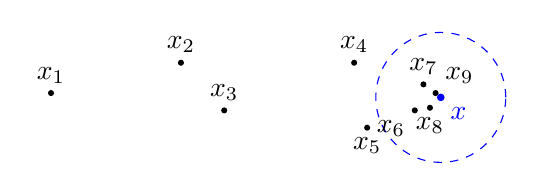
\begin{tikzpicture}[scale=0.55]
  % Limit point and its dashed neighborhood.
  \draw[blue, dashed] (0,0) circle (1.5);
  \fill[blue] (0,0) circle (2.5pt) node[blue, below right] {$x$};
  % Scattered approaching points x_1, x_2, ..., x_9.
  \fill (-9,0.1)      circle (2pt) node[above]      {$x_1$};
  \fill (-6,0.8)      circle (2pt) node[above]      {$x_2$};
  \fill (-5,-0.3)     circle (2pt) node[above]      {$x_3$};
  \fill (-2,0.8)      circle (2pt) node[above]      {$x_4$};
  \fill (-1.7,-0.7)   circle (2pt) node[below]      {$x_5$};
  \fill (-0.6,-0.3)   circle (2pt) node[below left] {$x_6$};
  \fill (-0.4,0.3)    circle (2pt) node[above]      {$x_7$};
  \fill (-0.25,-0.24) circle (2pt) node[below]      {$x_8$};
  \fill (-0.12,0.1)   circle (2pt) node[above right]{$x_9$};
\end{tikzpicture}
\end{document}
